%CLASSE DOCUMENTO - LINGUA E DIMENSIONE FONT
\documentclass[11pt]{toptesi}

%%%%%%%%%%%%%%%%%%%%%%%%%%%%%%%%%%%%%%%%%%%%%%%%%%%%%%%%%%%%%%%

% INCLUSIONE PACCHETTI
\usepackage[utf8]{inputenc} %utf8
\usepackage[italian]{babel}
\usepackage[T1]{fontenc}
\usepackage{blindtext}
\usepackage{graphicx,wrapfig}
\usepackage{booktabs}
\usepackage{lmodern}
\usepackage{varioref}
\usepackage{url}
\usepackage{array}
\usepackage{paralist}{\obeyspaces\global\let =\space}
\usepackage{verbatim} 
\usepackage{subfig}
\usepackage{tabularx}
\usepackage{amsmath}
\usepackage{amsfonts}
\usepackage{float}
\usepackage{amssymb}
\usepackage{multicol}
\usepackage{multirow}
\usepackage{listings}
\usepackage[pass]{geometry}
\usepackage[figuresright]{rotating}
\usepackage{algorithm}
\usepackage{algorithmic}
\usepackage{amsmath}
\usepackage[babel]{csquotes}
\usepackage{hyperref}
\usepackage[backend=bibtex]{biblatex}

%%%%%%%%%%%%%%%%%%%%%%%%%%%%%%%%%%%%%%%%%%%%%%%%%%%%%%%%%%%%%%%

% CONFIGURAZIONE LINK E RIFERIMENTI
\hypersetup{%
    pdfpagemode={UseOutlines},
    bookmarksopen,
    pdfstartview={FitH},
    colorlinks,
    linkcolor={black}, %COLORE DEI RIFERIMENTI AL TESTO
    citecolor={blue}, %COLORE DEI RIFERIMENTI ALLE CITAZIONI
    urlcolor={blue} %COLORI DEGLI URL
}

%%%%%%%%%%%%%%%%%%%%%%%%%%%%%%%%%%%%%%%%%%%%%%%%%%%%%%%%%%%%%%%

% CONFIGURAZIONE LISTATI/CODICE - CANCELLARE SE NON NECESSARIO
% PYTHON - BIANCO E NERO
\lstset{%
	captionpos=b,
	language=Python,
	basicstyle =\small\ttfamily,
	keywordstyle=\color{black}\bfseries,
	breaklines=true,
	breakatwhitespace=true,
	frame=lines,
	numbers=left,
	numberstyle=\footnotesize,
}

%%%%%%%%%%%%%%%%%%%%%%%%%%%%%%%%%%%%%%%%%%%%%%%%%%%%%%%%%%%%%%%

% FRENCHSPACING VA _SEMPRE_ ABILITATO PER DOCUMENTI IN ITALIANO
\frenchspacing

%%%%%%%%%%%%%%%%%%%%%%%%%%%%%%%%%%%%%%%%%%%%%%%%%%%%%%%%%%%%%%%

%DEFINIZIONE SEZIONI IN NUMERAZIONE ROMANA
%ELENCO DEI LISTATI/CODICI
\makeatletter
\newcommand\listofcodes{%
 \iffrontmatter\else\frontmattertrue\fi
 \if@openright\cleardoublepage\else\clearpage\fi
 % change the meaning of \chapter in a group
 \begingroup\def\chapter##1{\@schapter}
 \phantomsection % for the hyperlink
 \lstlistoflistings 
 \endgroup
} 
\makeatother

%%%%%%%%%%%%%%%%%%%%%%%%%%%%%%%%%%%%%%%%%%%%%%%%%%%%%%%%%%%%%%%

% INFORMAZIONI PDF - PERSONALIZZARE
\pdfinfo{%
  /Title    (Senza carta igienica)
  /Author   (Tinaso de Tinasis)
  /Subject  (Un trattato di toccante urgenza)
  /Keywords (LaTeXi carta igienica urgenza Politecnico Presicce)
}

%%%%%%%%%%%%%%%%%%%%%%%%%%%%%%%%%%%%%%%%%%%%%%%%%%%%%%%%%%%%%%%

% FRONTESPIZIO - PERSONALIZZARE
% ELIMINATE LE VOCI CHE NON VI SERVONO

% UNIVERSITA - NOME
\ateneo{Politecnico di Bari}

% FACOLTA - DICITURA - CANCELLARE O DECOMMENTARE
%\FacoltaDi{Faculty of}
% FACOLTA - NOME
\facolta{Ingegneria}


% CORSO DI LAUREA - DICITURA (MANTENERE LO SPAZIO) - CANCELLARE O DECOMMENTARE
%\CorsoDiLaureaIn{Master of Science in }
% CORSO DI LAUREA - NOME
\corsodilaurea{Ingegneria dell'Automazione}


% TIPOLOGIA TESI
\TesiDiLaurea{Tesi di Laurea Magistrale in Internet of Things}

% TITOLO
\titolo{Piattaforme di Crowdsourcing in sistemi IoT eterogenei}

% SOTTOTITOLO
\sottotitolo{Dipartimento di Ingegneria Elettrica e dell'Informazione}

% RELATORE/I - DICITURA - CANCELLARE SE UN SOLO RELATORE
%\AdvisorName{Relatori}
% RELATORE - PROF. NOME E COGNOME
\relatore{prof.\ Luigi Alfredo Grieco}
% RELATORE AGGIUNTIVO - PROF NOME E COGNOME
% SE SI HA SOLO UN RELATORE ELIMINARE INSIEME AD AdvisorName
\secondorelatore{prof.\ Giuseppe Piro}

% TUTORE AZIENDALE - TITOLO NOME E COGNOME
% \tutoreaziendale{Ing. Carlino Cane}
% TUTORE AZIENDALE - DICITURA//AZIENDA
% \NomeTutoreAziendale{Tutore Aziendale\\FeelGood Inc}


% CANDIDATO - NOME E COGNOME
\candidato{Antonio Brandi}


% LOGO UNIVERSITA
\logosede{images/logo_poliba}

% DATA - MESE ANNO
\sedutadilaurea{25 Luglio 2019}

%%%%%%%%%%%%%%%%%%%%%%%%%%%%%%%%%%%%%%%%%%%%%%%%%%%%%%%%%%%%%%%

% LISTA DEI CAPITOLI DA INCLUDERE - PERSONALIZZARE
\includeonly{%
chap_introduzione,%
chap_quo,%
chap_qua,%
chap_conclusioni,%
app_a,%
}

% FILE DI BIBLIOGRAFIA
\bibliography{bibliography} 


%%%%%%%%%%%%%%%%%%%%%%%%%%%%%%%%%%%%%%%%%%%%%%%%%%%%%%%%%%%%%%%

% INIZIO DOCUMENTO
\begin{document}

\frontespizio

%%%%%%%%%%%%%%%%%%%%%%%%%%%%%%%%%%%%%%%%%%%%%%%%%%%%%%%%%%%%%%%

%INTERLINEA - DEFAULT 1 - NON ESAGERATE, NON SUPERATE MAI 1.3 ;)
%\interlinea{1.2}

%%%%%%%%%%%%%%%%%%%%%%%%%%%%%%%%%%%%%%%%%%%%%%%%%%%%%%%%%%%%%%%

\frontmatter

% DEDICA - PERSONALIZZARE
 %VSPACE - PROPORZIONE USATA PER CENTRATURA VERTICALE DEL TESTO
 %FLUSHRIGHT - ALLINEAMENTO ORIZZONTALE A DESTRA
 \vspace*{\stretch{1}}
 \begin{flushright}
 \noindent
  
 \end{flushright}
 \vspace*{\stretch{6}}
\cleardoublepage


% CITAZIONE - PERSONALIZZARE
% VSPACE - PROPORZIONE USATA PER CENTRATURA VERTICALE DEL TESTO
% FLUSHRIGHT - ALLINEAMENTO ORIZZONTALE A DESTRA
\vspace*{\stretch{1}}
\begin{flushright}
\noindent
Solo coloro che sono abbastanza folli da pensare di cambiare il mondo,\\ alla fine lo cambiano per davvero

\textit{}
\end{flushright}
\vspace*{\stretch{6}}
\cleardoublepage
\vspace*{\stretch{1}}
\begin{flushright}
	\noindent
	\textit{}
\end{flushright}
\vspace*{\stretch{6}}
\cleardoublepage

%%%%%%%%%%%%%%%%%%%%%%%%%%%%%%%%%%%%%%%%%%%%%%%%%%%%%%%%%%%%%%%

% RINGRAZIAMENTI - PERSONALIZZARE
% \ringraziamenti
% Grazie a Grazia, Graziella e la sorella.

%%%%%%%%%%%%%%%%%%%%%%%%%%%%%%%%%%%%%%%%%%%%%%%%%%%%%%%%%%%%%%%

% ABSTRACT - PERSONALIZZARE
\sommario
In questo lavoro di tesi si intende esplorare le funzionalità e potenzialità offerte dalla rapida ascesa delle tecnologie disponibili nel mondo dell' Internet of Things. \\
A seguito di una dettagliata analisi dello stato dell'arte e dei campi di applicazione che maggiormente potrebbero beneficiare del rapido sviluppo delle tecnologie IoT, ci si concentrerà maggiormente sul settore della mobilità, con il fine ultimo di sviluppare un prototipo dimostrativo delle potenzialità offerte da una piattaforma di Crowdsourcing.\\
Nella fattispecie, l'intento della fase di prototipazione non sarà quello di descrivere dettagliatamente un prodotto finito o valido in tutte le circostanze, ma sarà piuttosto quello di mostrare quanto ampio può essere il mondo legato all'IoT e quanto semplice sia la scalabilità di un simile prototipo ad un mercato di massa, che non si limiti al solo settore della mobilità. \\
In ultima analisi, con riferimento al prototipo in output a questo lavoro di tesi, ne saranno mostrate le caratteristiche implementative, basate sullo standard Datex II. Il fine ultimo di questa fase sarà quello di mostrare la struttura implementativa del prototipo in funzione della quale poter fornire delle linee guida implementative e possibili sviluppi futuri.


%%%%%%%%%%%%%%%%%%%%%%%%%%%%%%%%%%%%%%%%%%%%%%%%%%%%%%%%%%%%%%%

% INDICI - ELIMINARE GLI INDICI NON NECESSARI

% INDICE GENERALE
\tableofcontents

% INDICE DELLE FIGURE
\listoffigures

% INDICE DELLE TABELLE
\listoftables

% INDICE DEI CODICI
\listofcodes

%%%%%%%%%%%%%%%%%%%%%%%%%%%%%%%%%%%%%%%%%%%%%%%%%%%%%%%%%%%%%%%

\mainmatter

% INCLUSIONE FILE CAPITOLI - PERSONALIZZARE - TENERE COERENTE CON LISTA IN ALTO
\chapter{Introduzione}
\label{chap:introduzione}


%This is a reference to a chapter \ref{chap:quo}. This is a reference to a figure \ref{fig:doge}. This is a reference to some code \ref{lst:hello}. This is a citation \cite{famous:paper}.
%
%\lstinputlisting[label=lst:hello, firstline=2, lastline=4, caption={I directly included a portion of a file}]{code/hello.py}
%
%\begin{lstlisting}[language=Java, label=lst:java, caption={Some code in another language than the default one}]
%public void prepare(AClass foo) {
%        AnotherClass bar = new AnotherClass(foo)
%}
%\end{lstlisting}
%
%\Blindtext

Il panorama mondiale ha, nell'ultimo decennio, riposto particolare attenzione ed interesse verso le emergenti tecnologie nel campo dell'Internet of Things. \\ Questo perchè, il paradigma IoT consente oggi di realizzare la vision ed il concept che era già stato supposto e predetto come sviluppo della rete Internet. Ovvero adempiere allo scopo di collegare il mondo. \\
Tuttavia, se grazie ad Interent è stato possibile collegare le persone, metterle in relazione, fornire ad essi gli strumenti per interagire tra loro, indipendentemente dalla loro posizione geografica o razza o sesso o colore, allo stesso modo, il naturale sviluppo di Internet non può che essere quello di mettere in relazione le cose. I dispositivi che siamo abituati ad utilizzare ogni giorno e che, seppur diversi ed eterogenei tra loro in termini di funzionalità, costo e posizione, sono in grado di comunicare tra loro, scambiarsi dati ed informazioni al fine di cambiare definitivamente il nostro modo di lavorare, acquistare, consumare e quindi di vivere.
\begin{figure}
\begin{center}
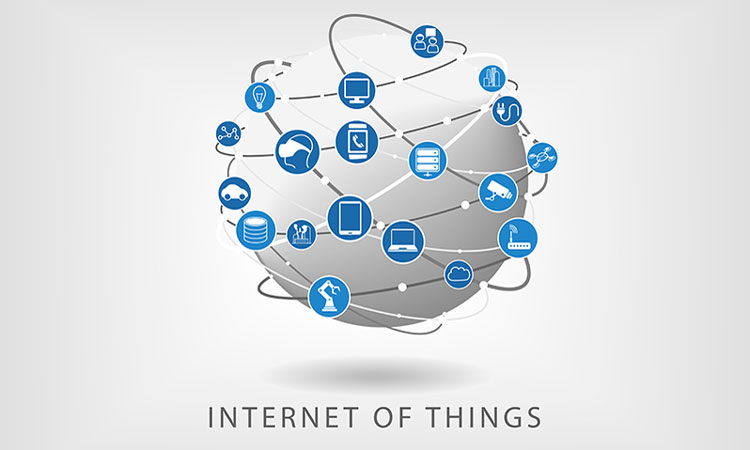
\includegraphics[width=0.7\columnwidth]{images/iot.jpg}
\end{center}
\caption{Overview del paradigma IoT}
\label{fig:iot}
\end{figure}

\section{IoT Enabling Technologies}
\label{sec:iot_enabling_technologies}

L'idea di una rete Internet che consentisse la comunicazione a livello globale tra persone o tra persone e cose o tra cose era già da molto tempo una visione condivsa di quello che sarebbe potuto essere lo sviluppo di Internet. \\
Tale visione è oggi possibile grazie alla diffusione capillare in qualsiasi strumento di piccoli, economici e potenti dispositivi di calcolo. \\
Tuttavia, affinchè una simile rivoluzione tecnologia si paventasse, era necessario superare i tradizionali protocolli di comunicazione tipici della rete Internet e creare conseguentemente delle nuove tecnologie per la comunicazione che fossero ottimizzate per le nuove esigenze.
Va infatti ricordato ancora una volta che la vision dell'IoT sia quella di abilitare una comunicazione tra qualsiasi tipo di dispositivo che abbia al suo interno una unità di calcolo. Questo significa stabilire una comunicazione tra dispositivi eterogenei, dispositivi che assolvono diversi compiti ed adempiono a diverse necessità e che sono molto spesso anche dotati di una diversa e limitata potenza di elaborazione. \\
Di qui la necessità di nuovi protocolli e tecnologie di comunicazione che non solo garantissero la comunicazione sicura di una grossa mole di dati tra un grande numero di dispositivi, ma che fossero anche dei protocolli leggeri dal punto di vista computazionale ed ovviamente economici, così da poter essere integrati in qualsiasi dispositivo, da quelli destinati all'industria a quelli destinati al mercato consumer.
Data la complessità della sfida tecnologica da fronteggiare e considerata l'eterogeneità del problema e delle necessità nei diversi campi applicativi,
sono stati sviluppati e proposti diverse tipologie di tecnologie e protocolli di comunicazione. \\
Tra le più rilevanti nel campo della comunicazione domestica o locale emergono Bluetooth Low Energy \cite{famous:paper_1} and Zigbee \cite{famous:paper_2}. Mentre altri protocolli come WiFi, LowPower Wide Area Networks (LPWA) \cite{famous:paper_3} e le comunicazioni cellulari come 3GPP , 4G o 5G \cite{famous:paper_Grieco_1} hanno uno scope più ampio, abilitando la comunicazione tra dispositivi anche molto distanti tra loro.



\chapter{Quo}
\label{chap:quo}
\Blindtext
\chapter{Qua}
\label{chap:qua}
\Blindtext
\chapter{Conclusioni}
\label{chap:conclusioni}
Attraverso il percorso di progettazione ed implementazione affrontato nel \autoref{chap:tre} e nel \autoref{chap:quattro}, si è giunti all'implementazione di un prototipo che mostri le principali componenti di una cloud application nel mondo dell'Internet of Things.\\
Il contributo che si è cercato di dare con questo lavoro di tesi è stato quello di mostare il processo logico e le motivazioni che abbiano portato ad alcune scelte progettuali che fossero poi riproducibili non solo in una particolare istanza, ma in tutte quelle applicazioni legate al mondo dell'IoT che condividano le stesse necessità e che, a prescindere dal loro scopo, abbiano una struttura comune.\\
La struttura, appunto, che è stata progettata ed implementata è sostanzialmente riconducibile a tre componenti fondamentali:
\begin{itemize}
	\item \textbf{Client Application:} Ovvero la applicazione e l'interfaccia che raccoglie e mostra i dati. In questo lavoro di tesi, l'interfaccia è un applicativo per smartphone Android. Tuttavia, le operazioni effettuate da questo applicativo sono eseguibili anche da qualsiasi altro dispositivo connesso in rete. Infatti, il suo compito sarà quello di raccogliere dati, inviare e ricevere dati attraverso Internet ed infine mostrare i dati. Si può pensare ad infinite altre soluzioni che siano in grado di riprodurre questi compiti e che quindi possano sostituire la client application implementata in questo lavoro di tesi per addattarsi a nuove necessità.
	
	\item \textbf{Server Application:} Ovvero la architettura del Server che è in ascolto e riceve i dati inviati dai client. In questo lavoro di tesi, per l'implementazione della Server application ci si è affidati ad un servizio esterno fornito da Amazon Web Services chiamato IoT Core. Anche in questo caso, i compiti che la server application deve svolgere sono, nella maggior parte, riproducibili da qualsiasi altro servizio cloud offerto da altre compagnie e perfino da servizi cloud implementati privatamente. I compiti ai quali dovrà assolvere una server application saranno infatti: autenticazione della comunicazione, implementazione di uno standard di comunicazione comune con i client, implementazione di una comunicazione publisher/subscriber con il client ed infine automatizzazione del processo di salvataggio dei dati ricevuti all'interno di un database.
	
	\item \textbf{Database Architecture and Data Analysis:} Strettamente collegata alla server application vi è anche la architettura del database nella quale memorizzare i dati raccolti ed eventualmente già filtrati dalla server application. Anche in questo caso, per l'implementazione di questo servizio, ci si è affidati ad un servizio esterno fornito da Amazon Web Services chiamato DynamoDB. Ma ancora, i compiti assolti da questo servizio sono riproducibili da altri servizi offerti da altre compagnie e perfino da databases gestiti localmente e privatamente. Infatti, il Database dovrà : consentire l'inserimento di nuovi elementi, consentire l' interrogazione di elementi già presenti, fornire delle interfacce per l'analisi dei dati contenuti al suo interno. 
\end{itemize}

Proprio focalizzandosi su queste poche componenti dell'architettura di una cloud application, si è dato un esempio implementativo di ognuna per lo sviluppo del sistema di raccolta dati relativi ad eventi stradali. \\
Sebbene si renda necessaria una successiva fase di 'ingegnerizzazione' di questo prototipo, i suoi utilizzi possono avere un impatto molto forte sul settore dell'automotive, già soggetto ad una vera e propria rivoluzione. Con una applicazione simile a quella prototipata in questo lavoro di tesi, si potrebbe infatti avere una sorta di scatola nera in ogni veicolo che attraversa la rete stradale e che quindi raccoglie miliardi di dati in frazioni di secondo. Ulteriormente, l'unione di questi dati e la loro analisi attraverso algoritmi di Machine Learning, potrebbero suppoprtare lo sviluppo e l'efficacia delle auto a guida autonoma. Tutto questo, al costo di uno smartphone.\\



\appendix
% INCLUSIONE APPENDICI - - PERSONALIZZARE - TENERE COERENTE CON LISTA IN ALTO
\chapter{Utilizzo del Protocollo DATEX II}
\label{app:a}
In questo appendice sono mostrati  i diagrammi delle classi relativi all'utilizzo del Protocollo DATEX II all'interno del sistema definito nel \autoref{chap:tre}.\\
I diagrammi delle classi di seguito mostrati sono stati ricavati da quelli progettati per lo standard DATEX. (\url{http://d2docs.ndwcloud.nu/_static/umlmodel/v3.0/index.htm})\\
Si presti inoltre attenzione al fatto che i diagrammi delle classi mostrati in questo appendice non coprono il progetto nella sua interezza ma si intendono riferite alla sola implementazione dello standard DATEX II all'interno del progetto.
Infine, i diagrammi delle classi di seguito esposti non comprendono lo standard DATEX II nella sua interezza, ma riguardano le sole componenti che si è ritenuto opportuno integrare nel progetto.\\
\subsubsection{General Structure}
\begin{figure}
	\begin{center}
		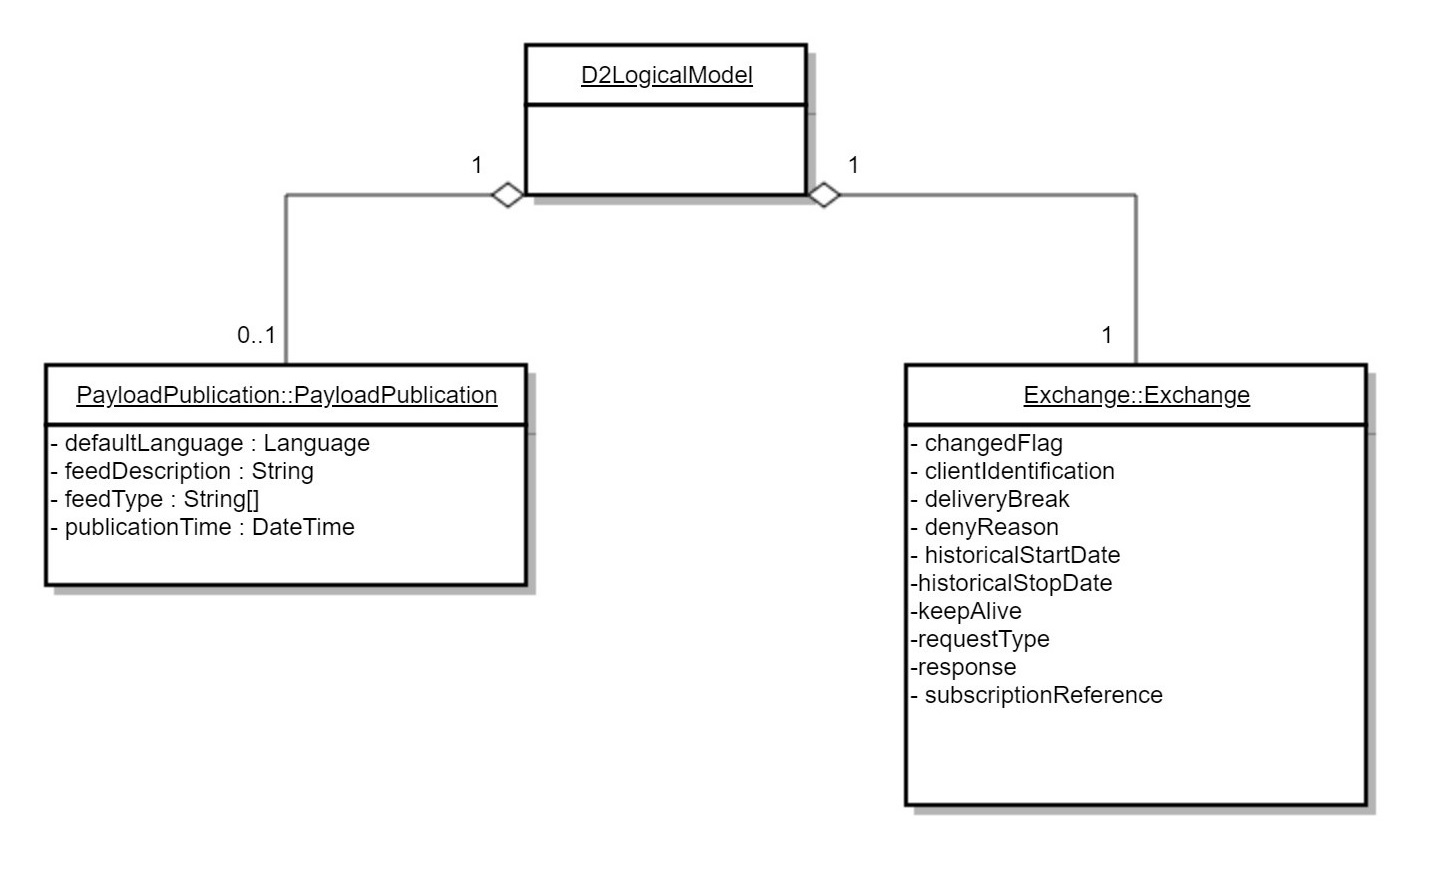
\includegraphics[width=0.6\columnwidth]{images/uml_1}
	\end{center}
	\caption{Distinzione effettuata dallo Standard DATEX II tra metodo di comunicazione (\textit{Exchange}) e formato del Payload (\textit{PayloadPublication})}
	\label{fig:app_uml_1}
\end{figure}
\begin{figure}
	\begin{center}
		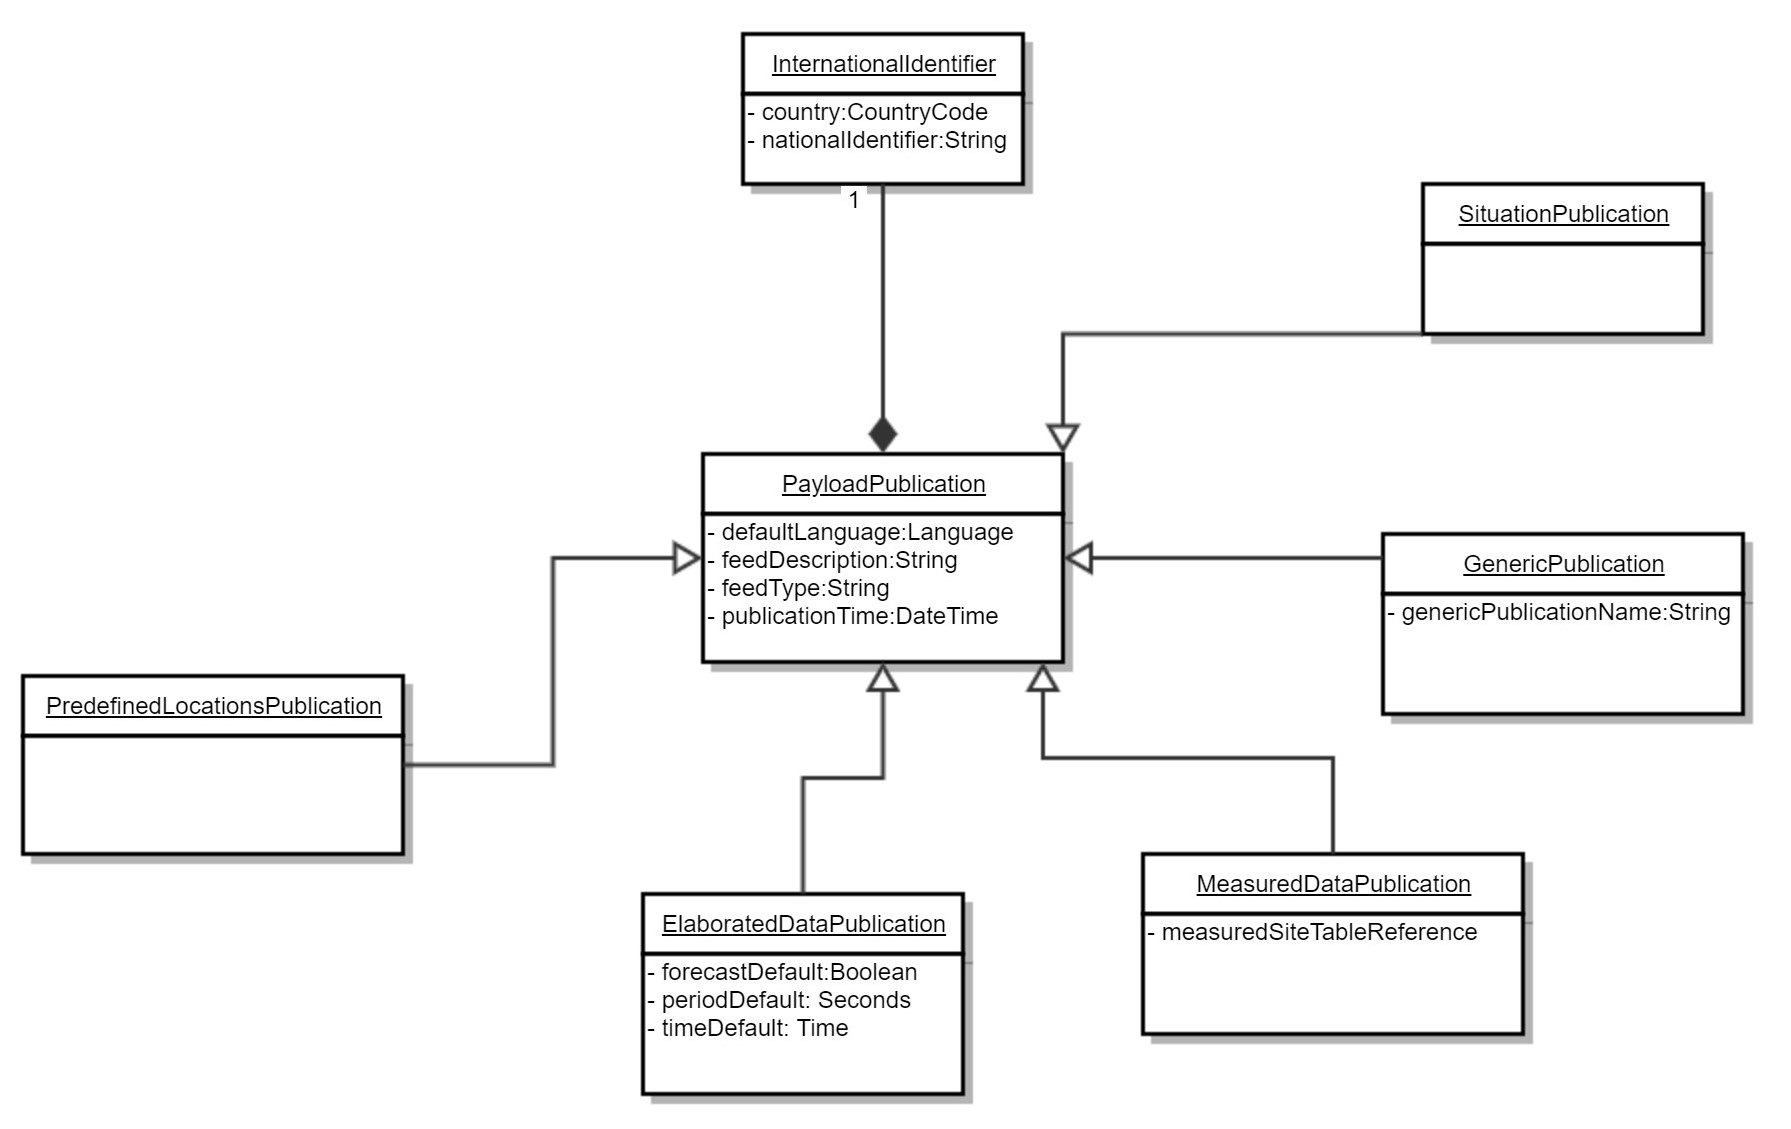
\includegraphics[width=0.9\columnwidth]{images/datexii_publication_implementation}
	\end{center}
	\caption{Implementazione della Publication}
	\label{fig:app_datexii_publication_implementation}
\end{figure}
\begin{figure}
	\begin{center}
		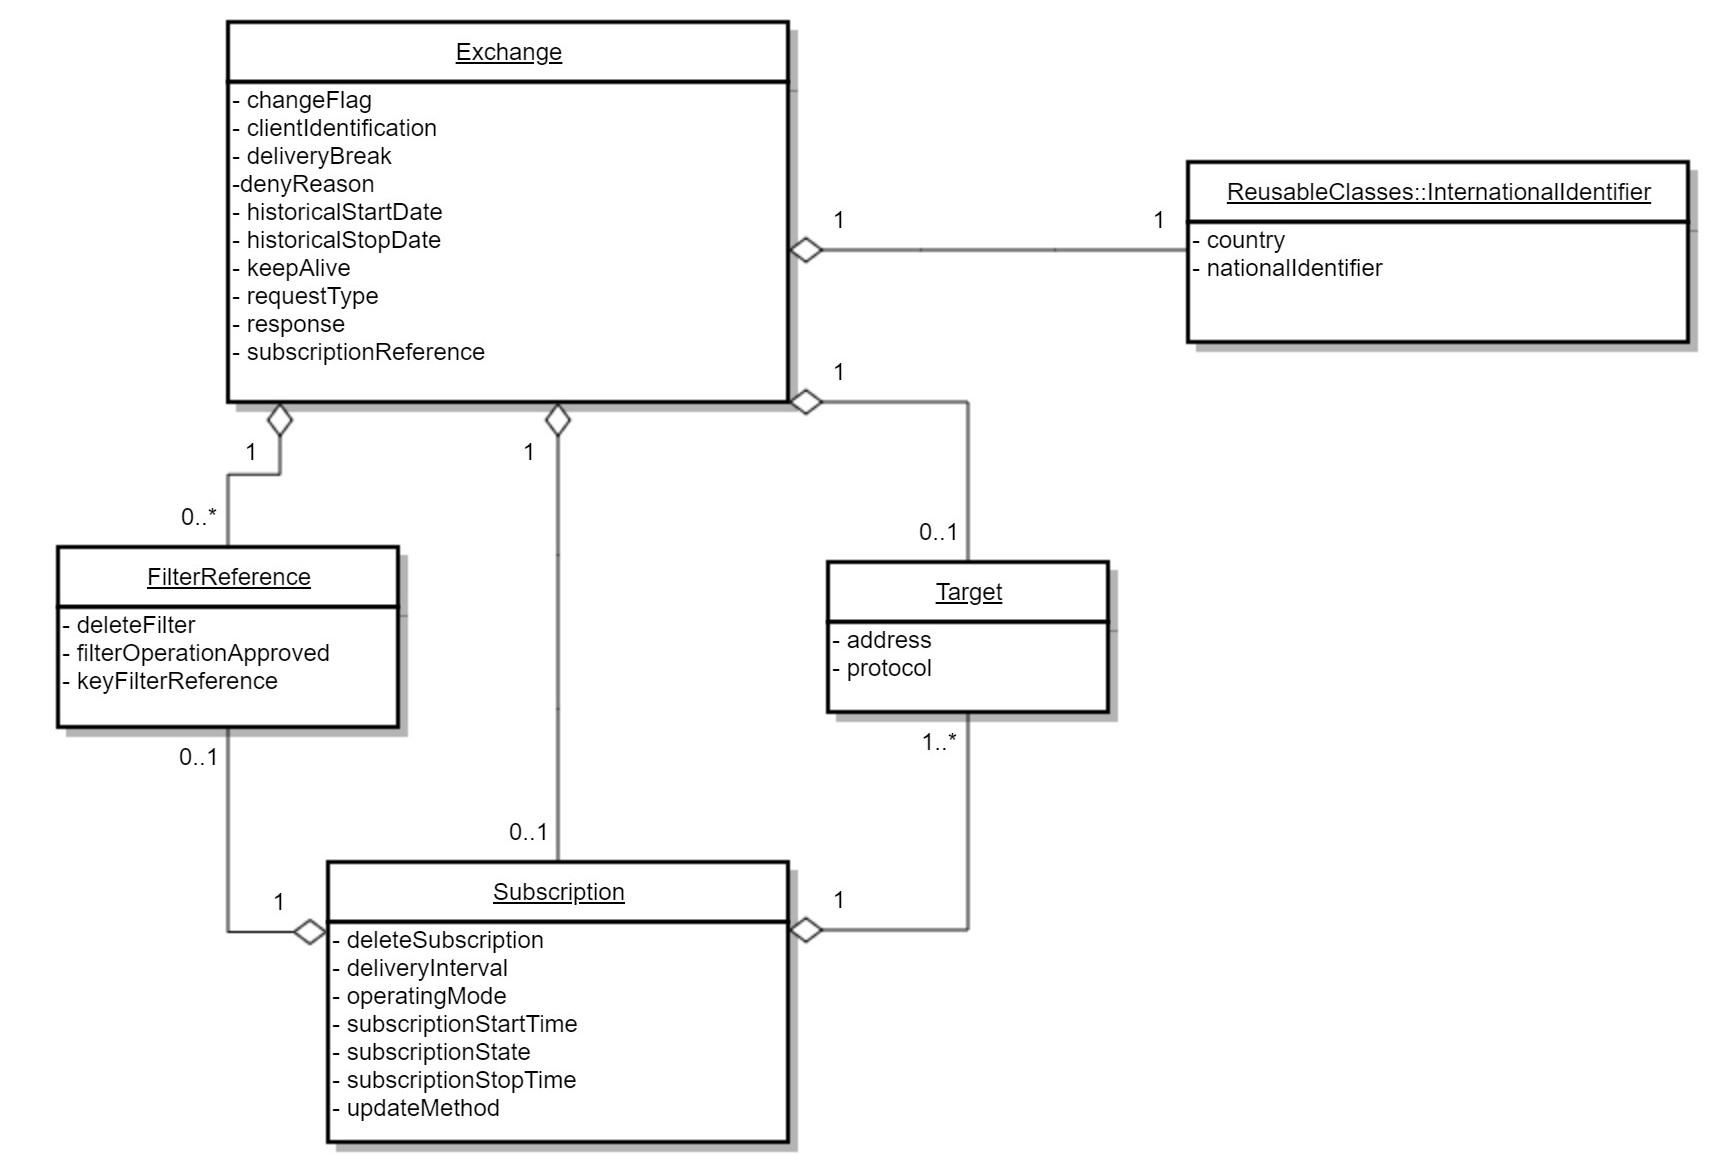
\includegraphics[width=0.8\columnwidth]{images/uml_2}
	\end{center}
	\caption{Implementazione del' Exchange}
	\label{fig:app_uml_2}
\end{figure}
\subsubsection{Location}
\begin{figure}
	\begin{center}
		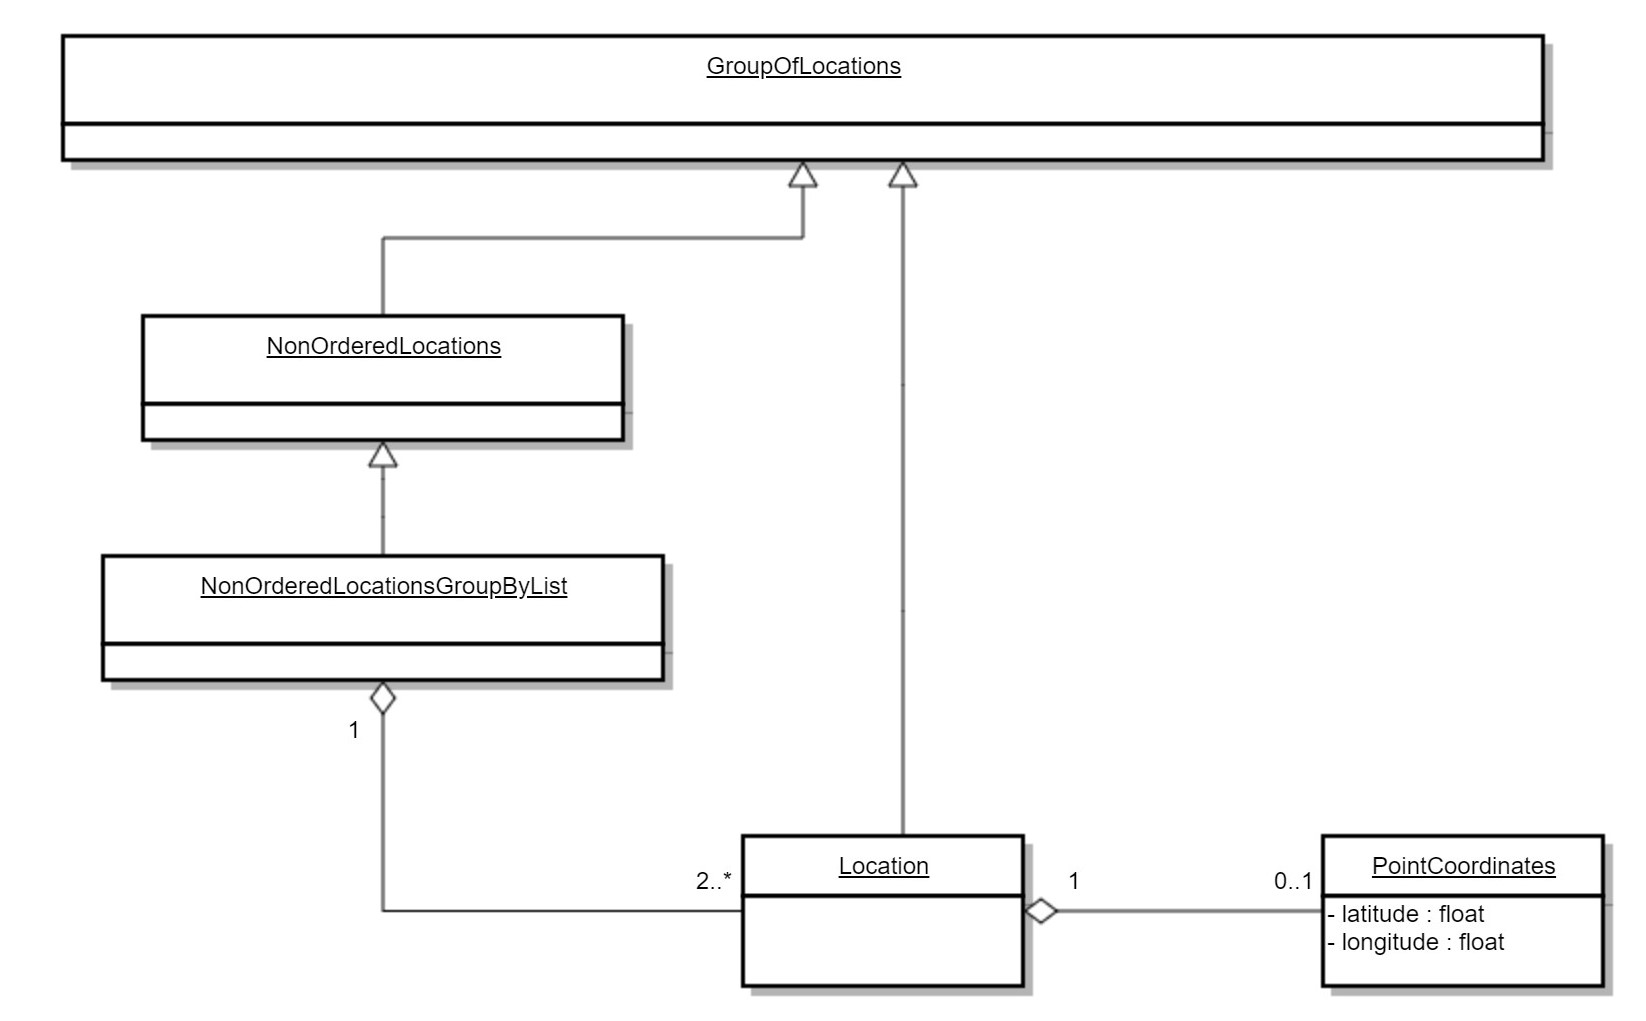
\includegraphics[width=1\columnwidth]{images/uml_3_3}
	\end{center}
	\caption{Location reference}
	\label{fig:app_uml_3_3}
\end{figure}
\subsubsection{Elaborated Data Publication}
\begin{figure}
	\begin{center}
		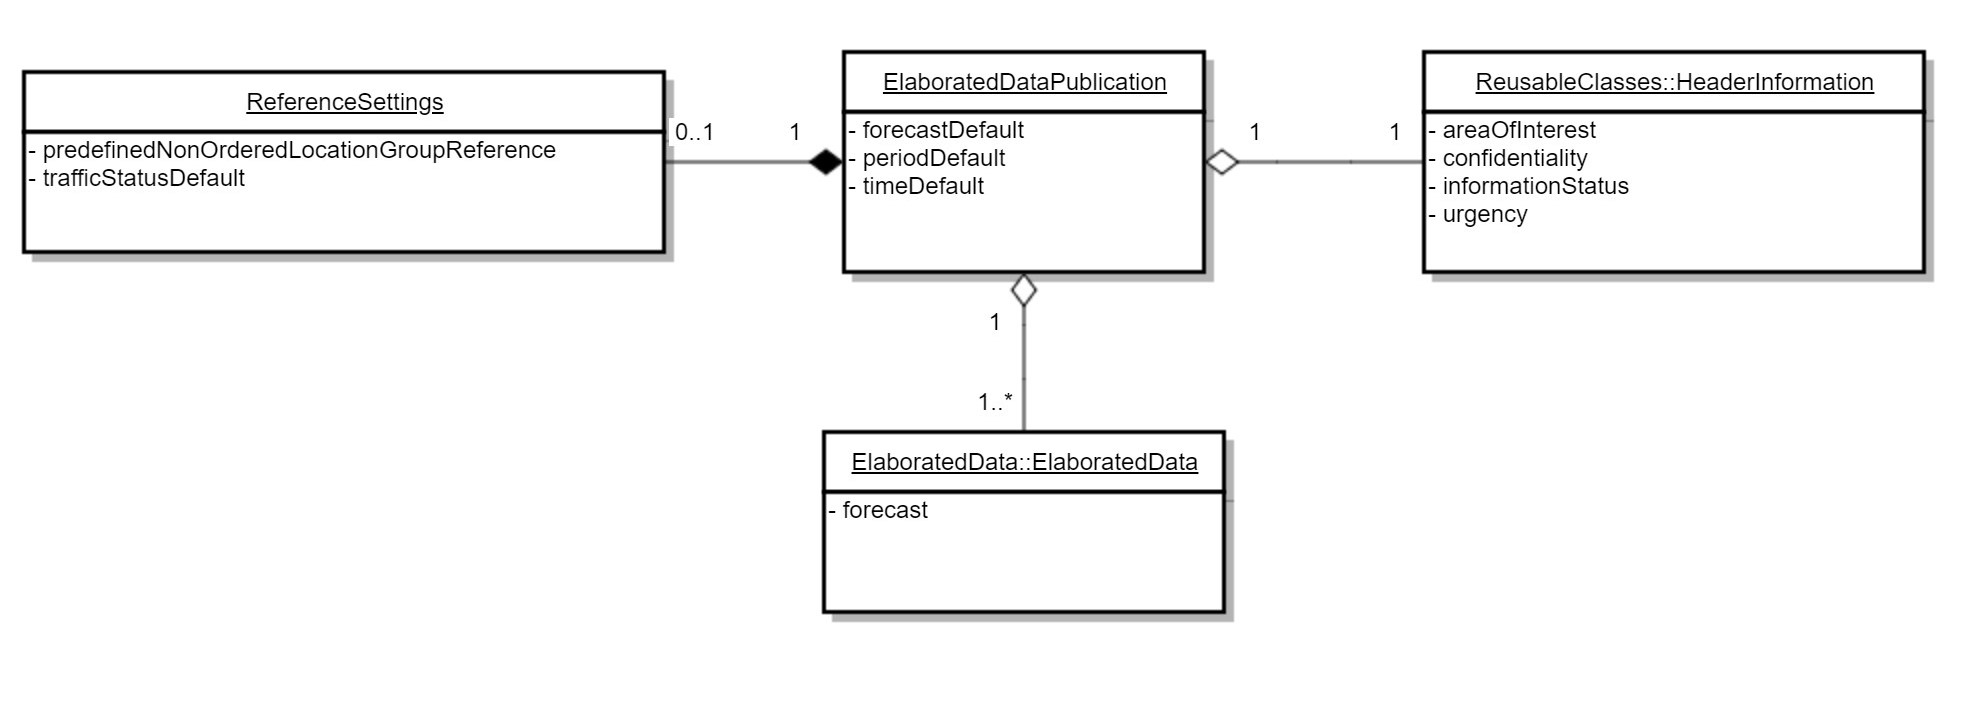
\includegraphics[width=1\columnwidth]{images/uml_3_6}
	\end{center}
	\caption{Elaborated Data Publication structure}
	\label{fig:app_uml_3_6}
\end{figure}
\begin{figure}
	\begin{center}
		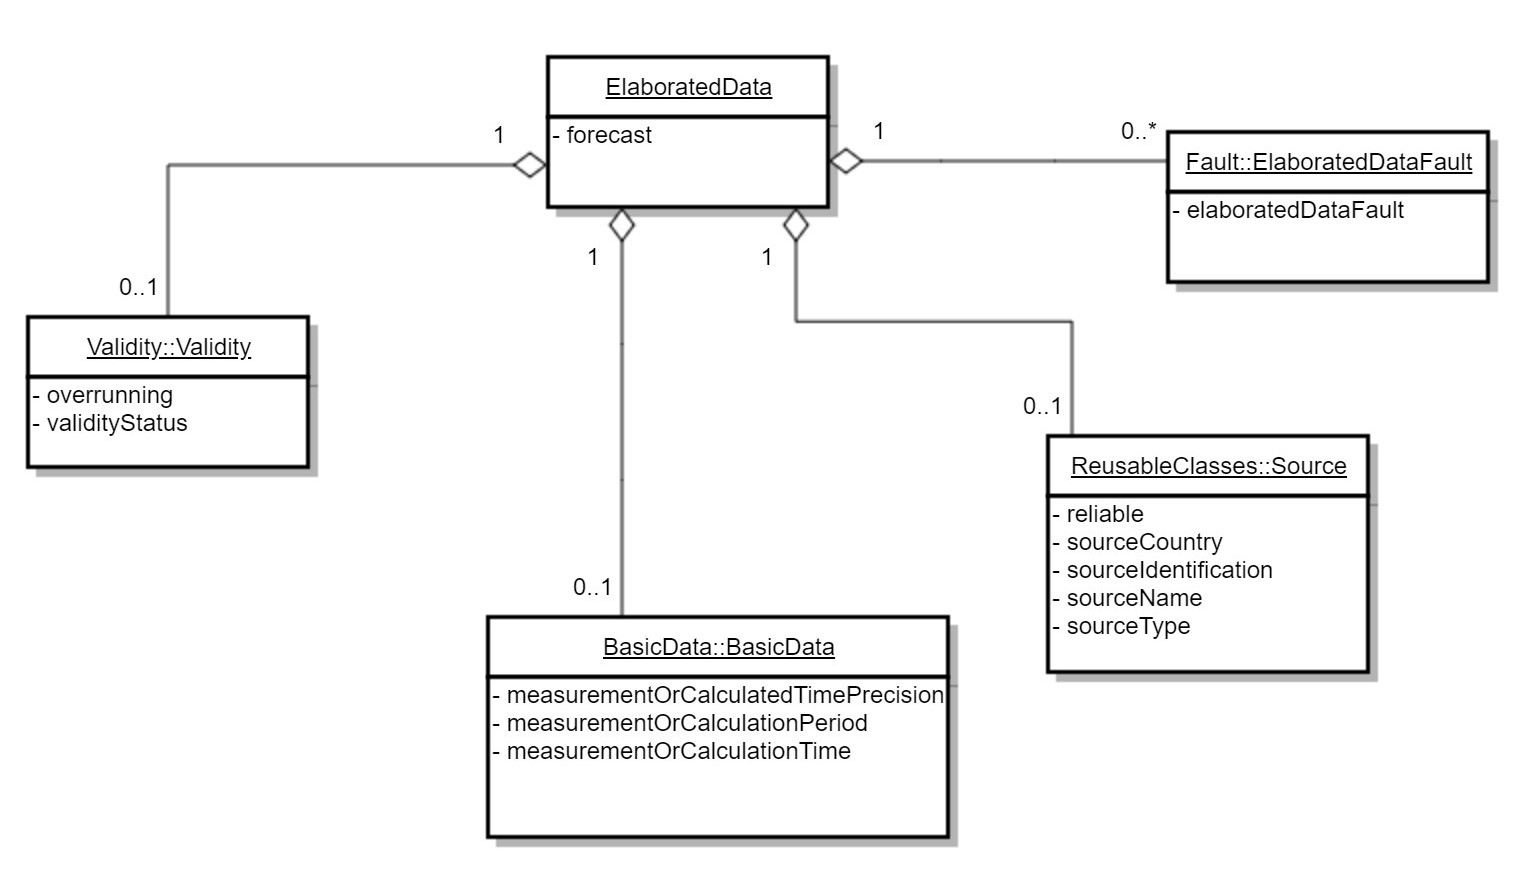
\includegraphics[width=0.7\columnwidth]{images/uml_4_30}
	\end{center}
	\caption{Elaborated Data Implementation}
	\label{fig:app_uml_4_30}
\end{figure}
\subsubsection{Measured Data Publication}
\begin{figure}
	\begin{center}
		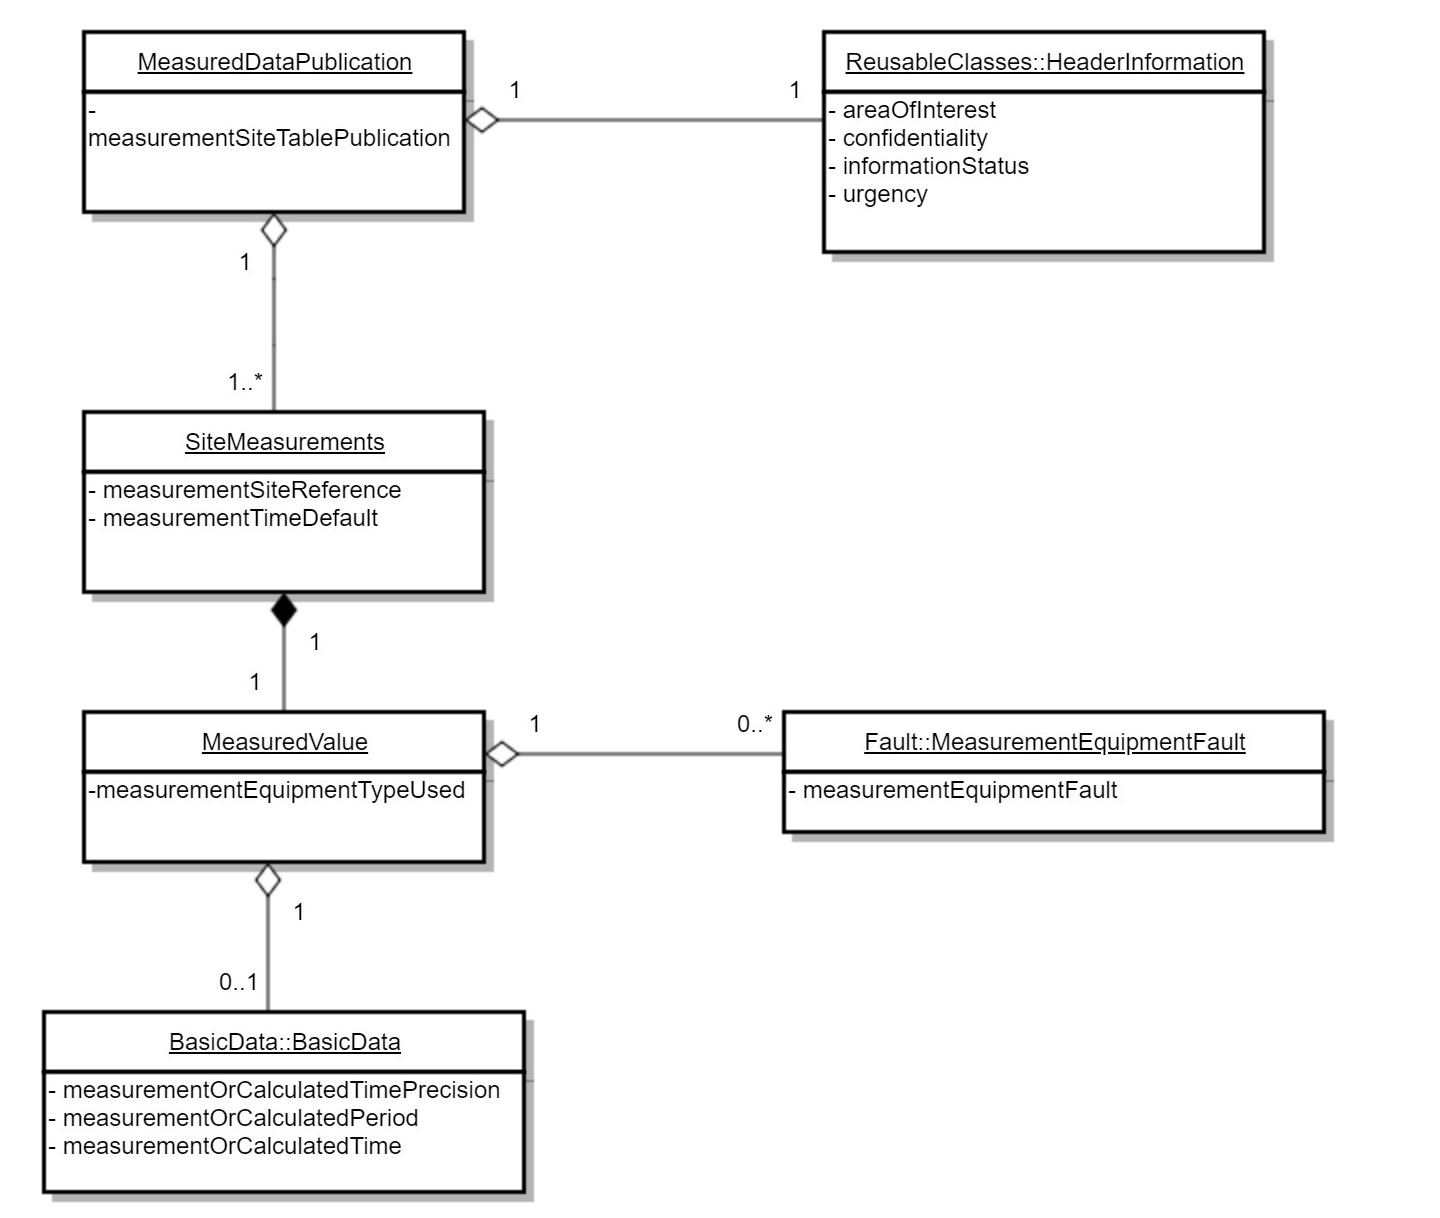
\includegraphics[width=0.8\columnwidth]{images/uml_3_8}
	\end{center}
	\caption{Measured Data Structure}
	\label{fig:app_uml_3_8}
\end{figure}
\begin{figure}
	\begin{center}
		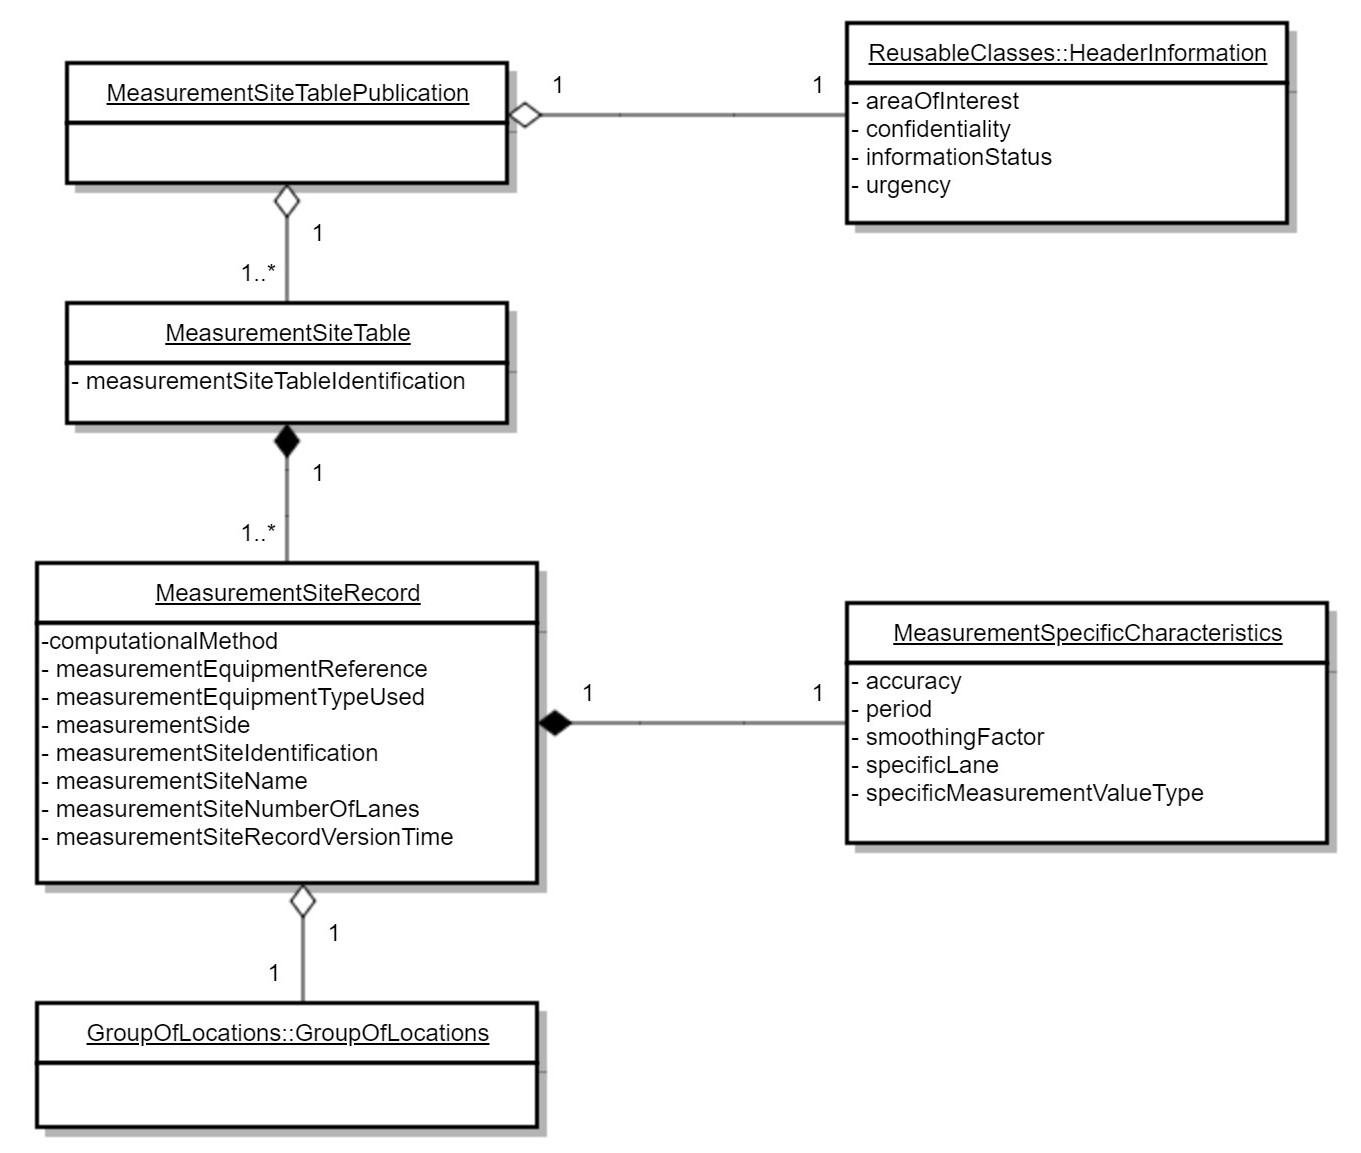
\includegraphics[width=0.75\columnwidth]{images/uml_3_9}
	\end{center}
	\caption{Measurement Site Record Structure}
	\label{fig:app_uml_3_9}
\end{figure}
\begin{figure}
	\begin{center}
		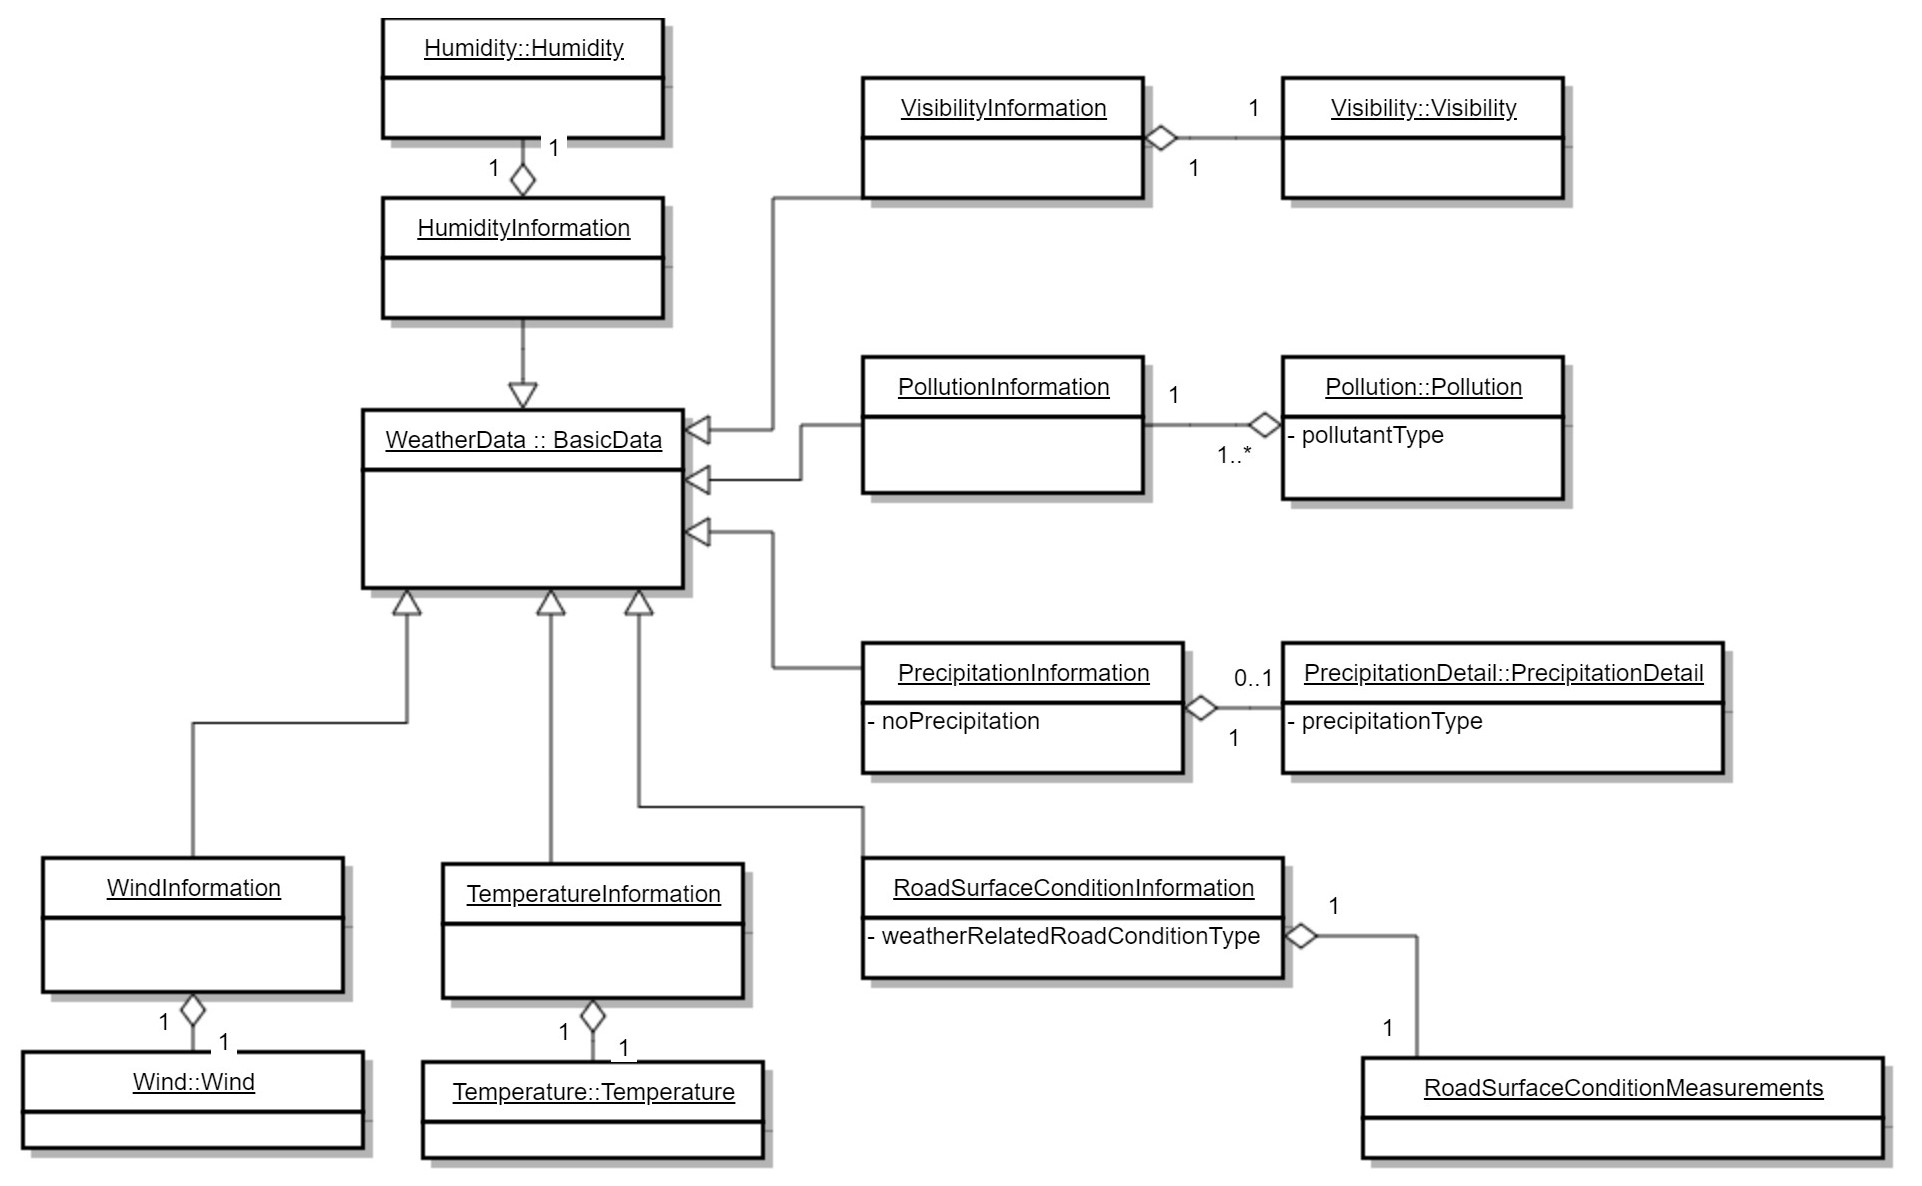
\includegraphics[width=0.8\columnwidth]{images/uml_4_28}
	\end{center}
	\caption{Basic Data Default Implementation}
	\label{fig:app_uml_4_28}
\end{figure}
\begin{figure}
	\begin{center}
		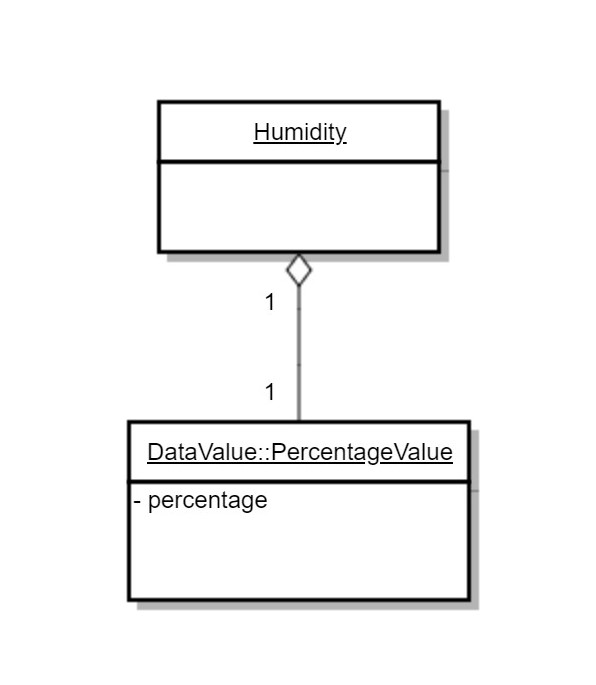
\includegraphics[width=0.5\columnwidth]{images/uml_5_14}
	\end{center}
	\caption{Humidity Implementation}
	\label{fig:app_uml_5_14}
\end{figure}
\begin{figure}
	\begin{center}
		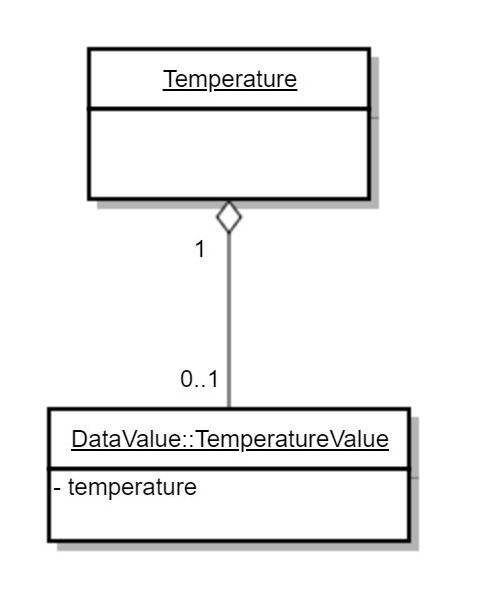
\includegraphics[width=0.45\columnwidth]{images/uml_5_18}
	\end{center}
	\caption{Temperature Implementation}
	\label{fig:app_uml_5_18}
\end{figure}
\begin{figure}
	\begin{center}
		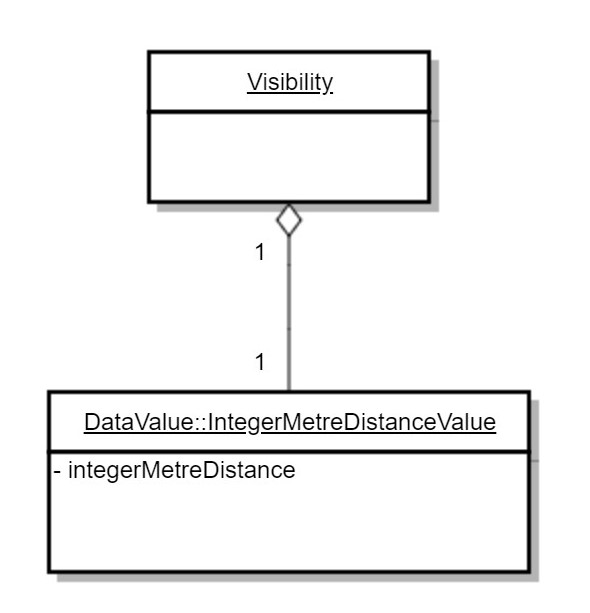
\includegraphics[width=0.65\columnwidth]{images/uml_5_19}
	\end{center}
	\caption{Visibility Implementation}
	\label{fig:app_uml_5_19}
\end{figure}
\begin{figure}
	\begin{center}
		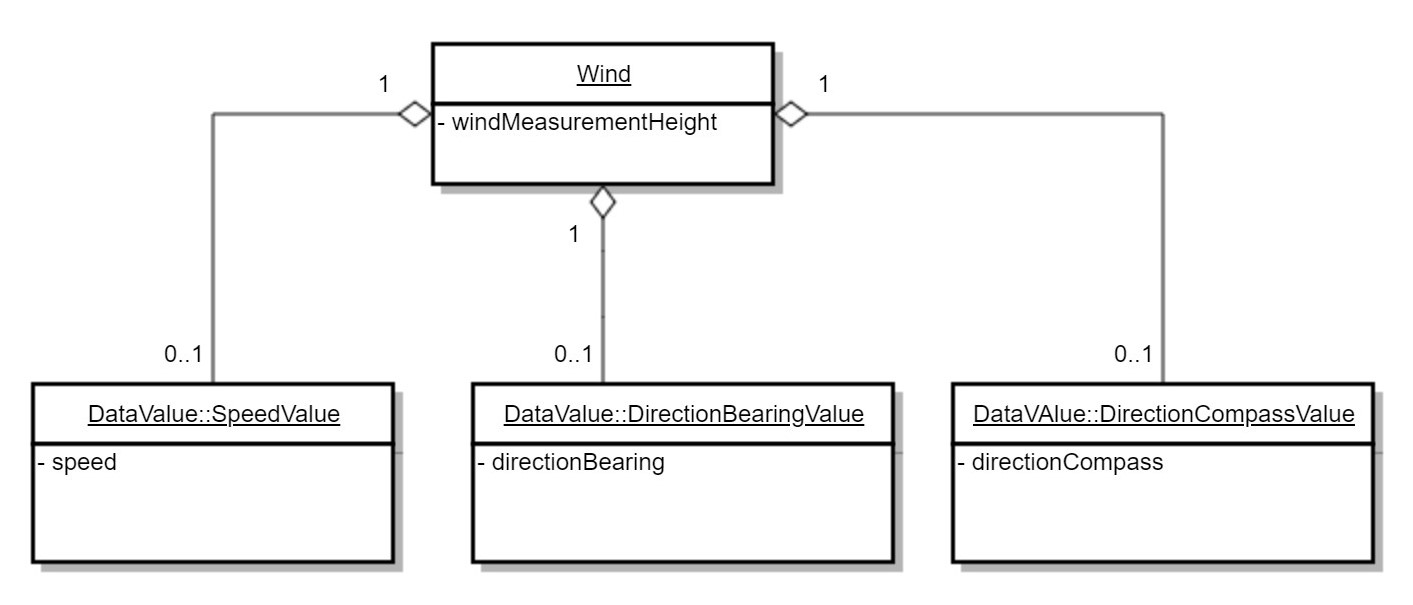
\includegraphics[width=1.1\columnwidth]{images/uml_5_20}
	\end{center}
	\caption{Wind Implementation}
	\label{fig:app_uml_5_20}
\end{figure}
\subsubsection{Situation Publication}
\begin{figure}
	\begin{center}
		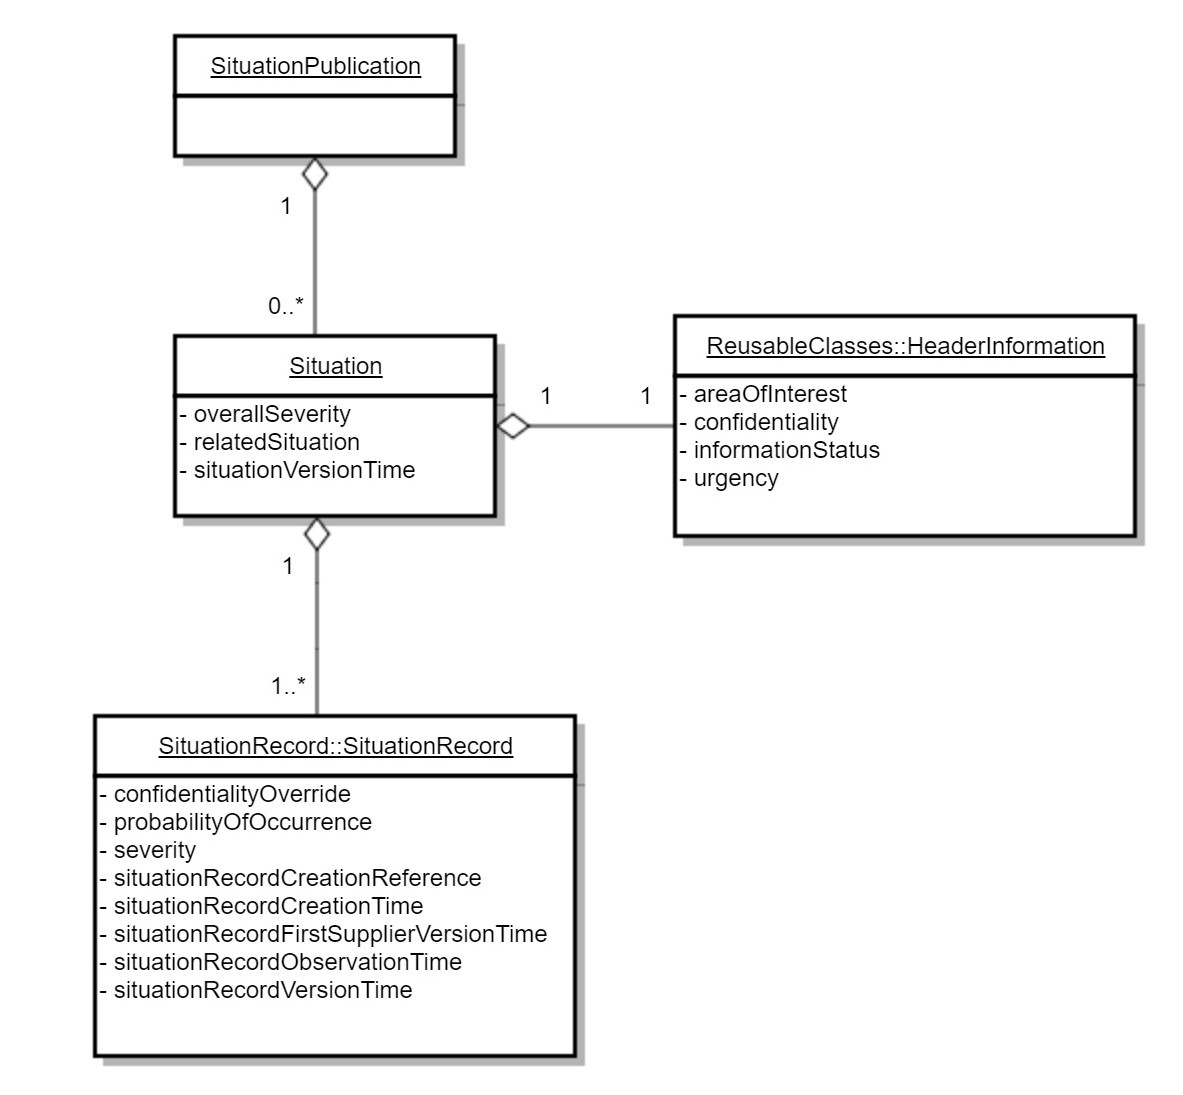
\includegraphics[width=0.7\columnwidth]{images/uml_3_11}
	\end{center}
	\caption{Situation Publication Structure}
	\label{fig:app_uml_3_11}
\end{figure}
\begin{figure}
	\begin{center}
		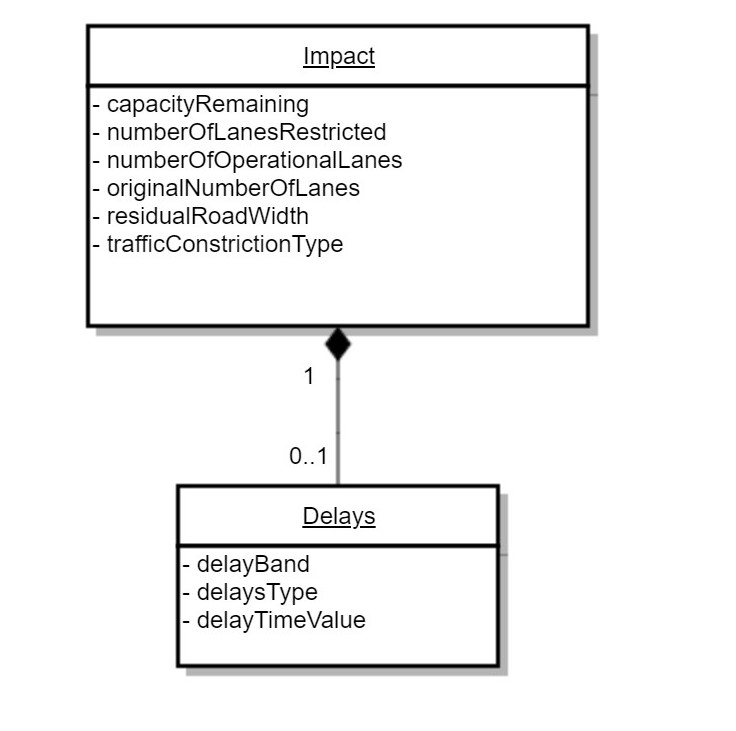
\includegraphics[width=0.45\columnwidth]{images/uml_4_32}
	\end{center}
	\caption{Impact Implementation}
	\label{fig:app_uml_4_32}
\end{figure}
\begin{figure}
	\begin{center}
		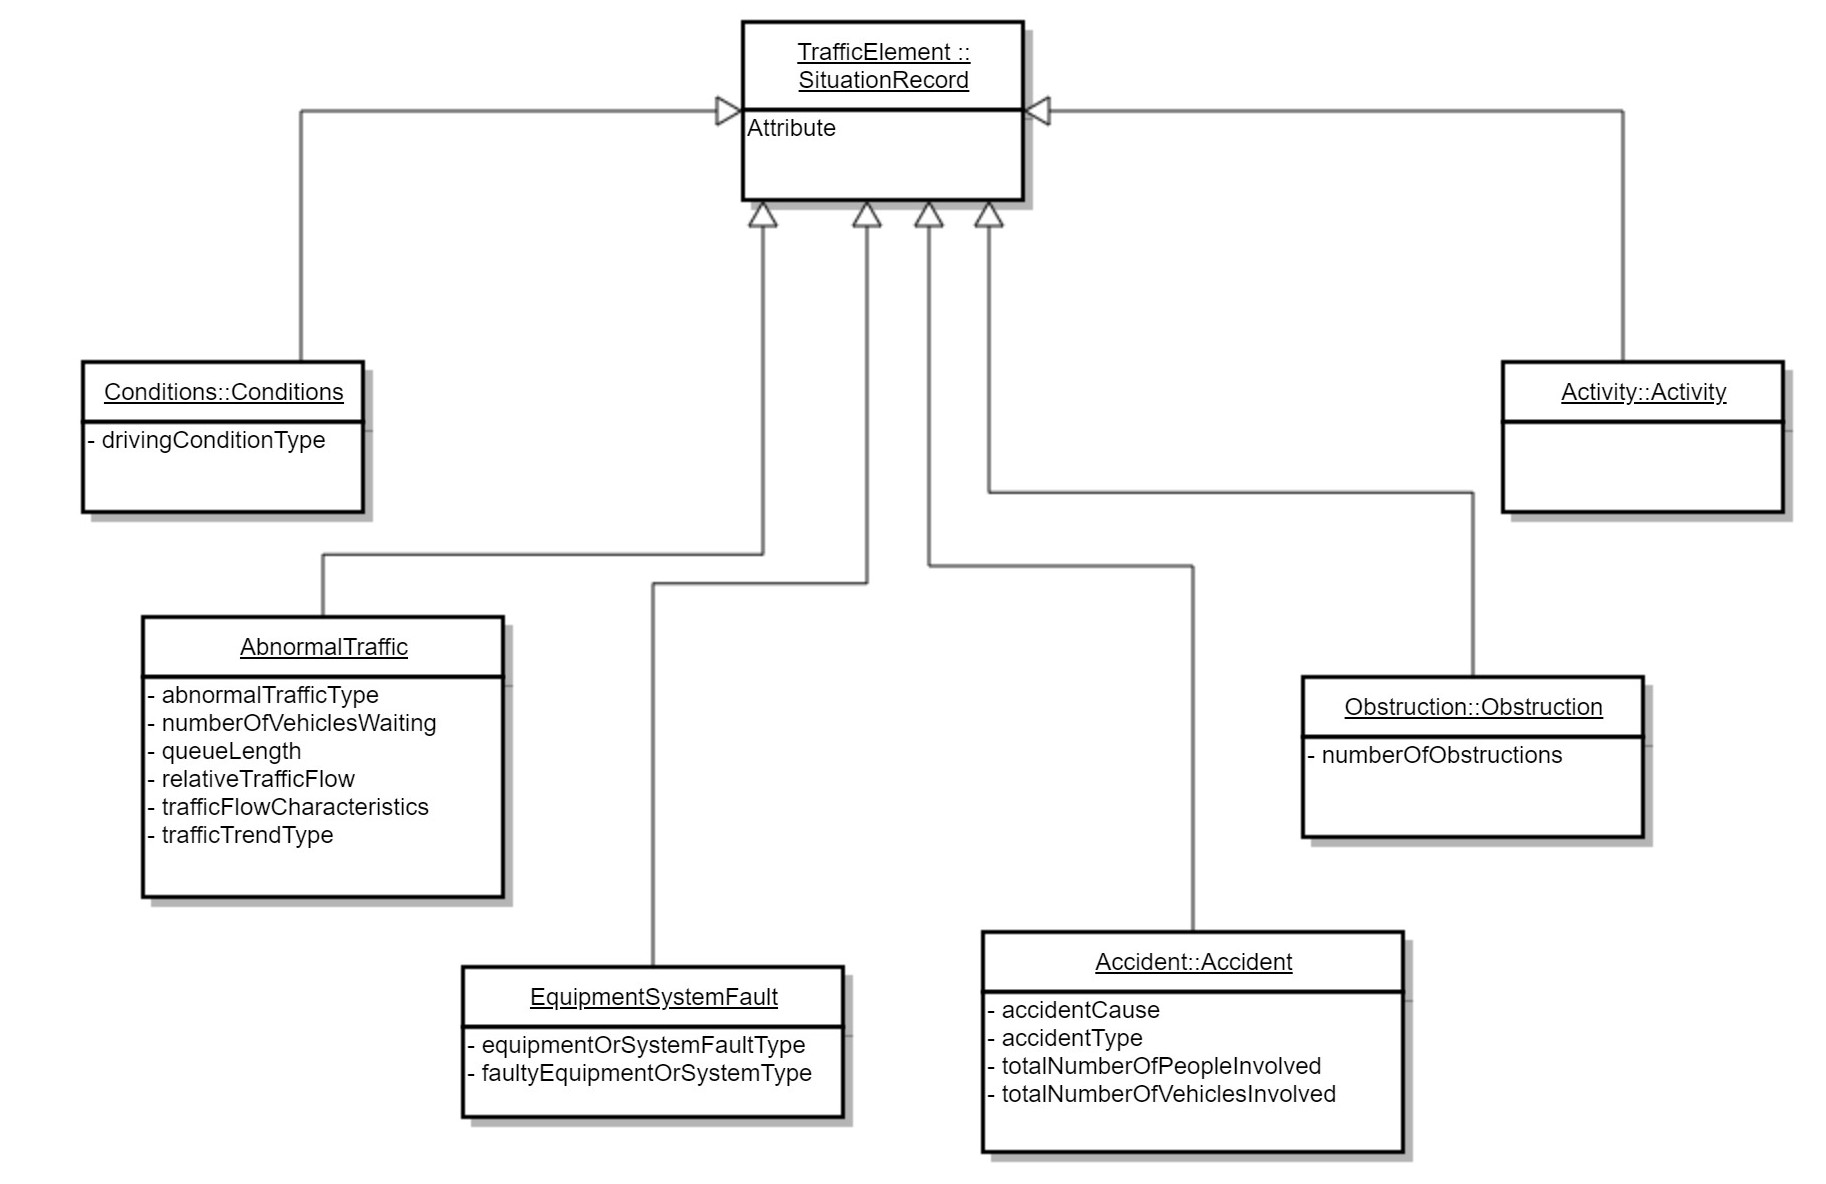
\includegraphics[width=0.85\columnwidth]{images/uml_4_36}
	\end{center}
	\caption{Traffic Element Implementation}
	\label{fig:app_uml_4_36}
\end{figure}
\begin{figure}
	\begin{center}
		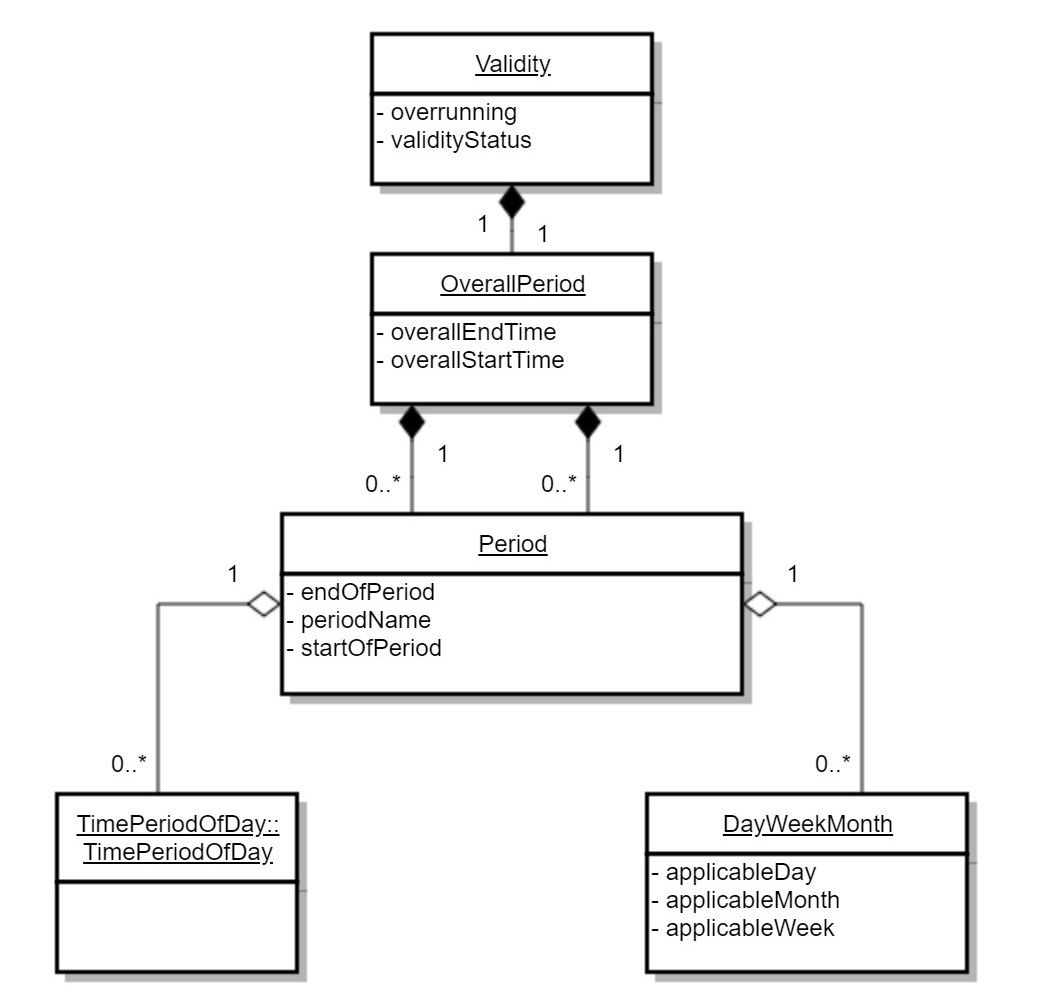
\includegraphics[width=0.6\columnwidth]{images/uml_4_37}
	\end{center}
	\caption{Validity Implementation}
	\label{fig:app_uml_4_37}
\end{figure}
\subsubsection{Standard Extension}
\begin{figure}
	\begin{center}
		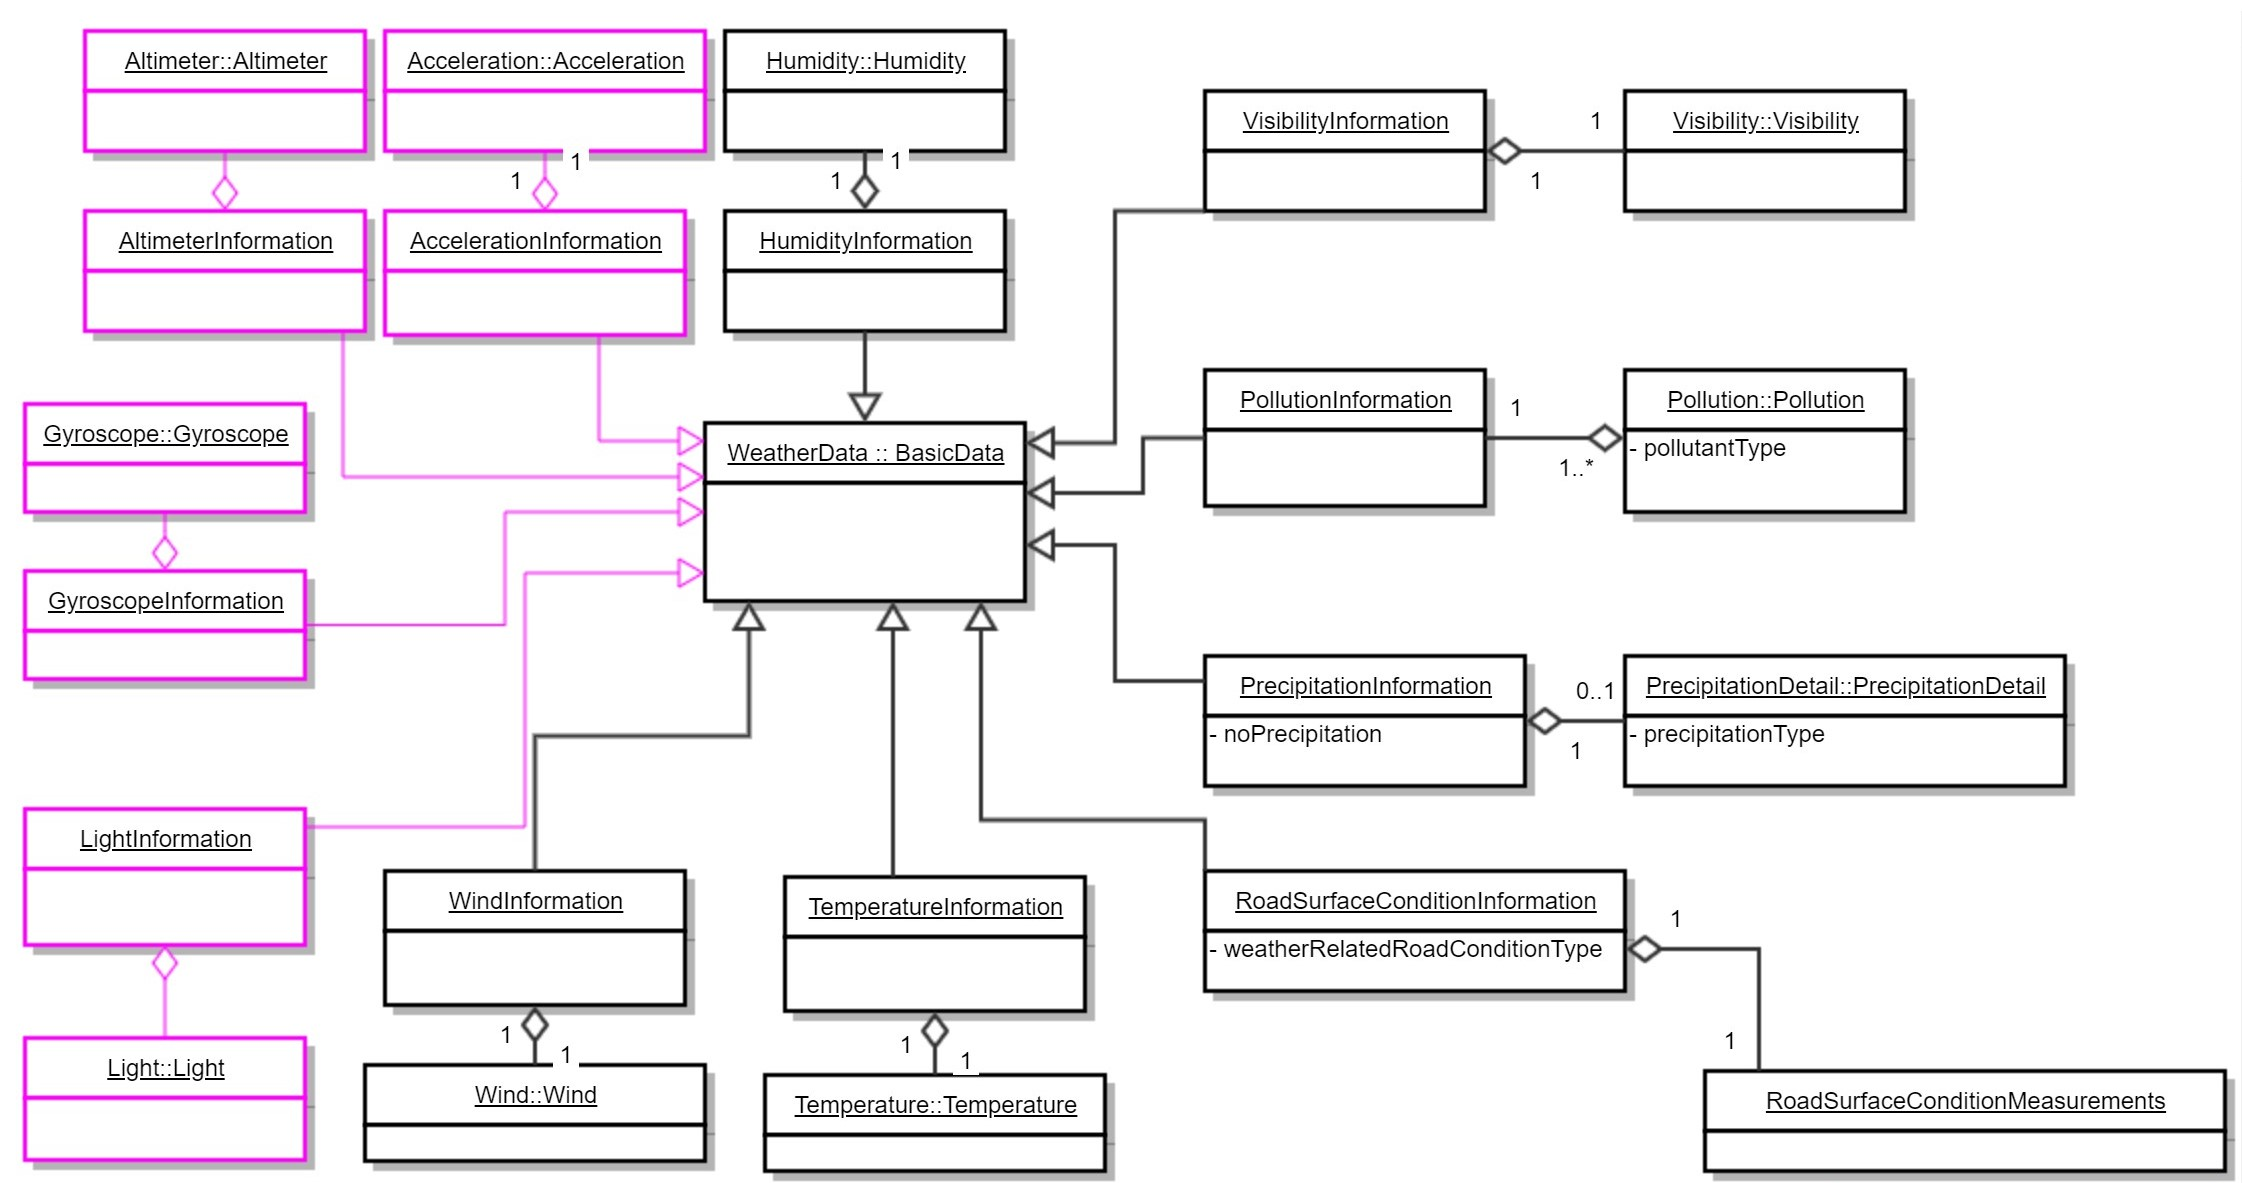
\includegraphics[width=1\columnwidth]{images/uml_4_28_extended}
	\end{center}
	\caption{Level B extension to the DATEX II Standard}
	\label{fig:app_uml_4_28_extended}
\end{figure}



%%%%%%%%%%%%%%%%%%%%%%%%%%%%%%%%%%%%%%%%%%%%%%%%%%%%%%%%%%%%%%%

% BIBLIOGRAFIA
\phantomsection
\addcontentsline{toc}{chapter}{\refname}
\nocite{*}
\printbibliography

\end{document}